\newcommand{\covtype}{\texttt{covtype}\xspace}
\newcommand{\sensit}{\texttt{sensit}\xspace}

% no longer in use
\newcommand{\resultcurves}[2]{
\begin{figure}[!h]
\centering
\subfigure[\covtype.]{\includegraphics[width=0.22\textwidth]{#1_covtype_pu_resvm.pdf}}\qquad
\subfigure[\sensit.]{\includegraphics[width=0.22\textwidth]{#1_sensit_2_semi_resvm.pdf}}\\
\caption{#2}
\label{fig:results-#1}
\end{figure}
}

\newcommand{\resultcurvesnew}[2]{
\begin{figure}[!h]
\centering
%\subfigure[Rank CDF for \covtype.]{\includegraphics[width=0.2\textwidth]{cdf_covtype_pu_resvm.pdf}}\qquad
%\subfigure[ROC curves for \covtype.]{\includegraphics[width=0.2\textwidth]{roc_covtype_pu_resvm.pdf}}\qquad
%\subfigure[PR curves for \covtype.]{\includegraphics[width=0.2\textwidth]{pr_covtype_pu_resvm.pdf}}
\subfigure[Rank CDF for \covtype.]{\includegraphics[width=0.2\textwidth]{#1_cdf.pdf}}\qquad
\subfigure[ROC curves for \covtype.]{\includegraphics[width=0.2\textwidth]{#1_roc.pdf}}\qquad
\subfigure[PR curves for \covtype.]{\includegraphics[width=0.2\textwidth]{#1_pr.pdf}}
\caption{#2}
\label{fig:results-#1}
\end{figure}
}

\section{Results and discussion} \label{results}
%To demonstrate the applicability and robustness of our approach, we show the resulting estimates of ROC and PR curves on two public data sets in a PU learning setting and compare our estimates to the truth.\footnote{Python scripts and data to reproduce the results are provided in the supplementary material. We will publicly release the code after acceptance.}
%
%We used rankings and corresponding true labels of simulations done by BLINDED, in which classifiers were tuned and trained in a PU learning context and tested on an independent, fully labeled test set. Since all test labels are available, this enables us to compute the true curves as a reference. We used the rankings produced by the approach introduced in BLINDED on the \covtype and \sensit data sets \citep{Blackard00covtype, duarte2004vehicle}. The \covtype test set consists of $20,000$/$20,000$ positives/negatives and the \sensit test set consists of $5,250$/$14,455$ positives/negatives.
%
%In our estimations, we discarded all negative labels and $90\%$ of positive labels (at random). This setup yields $|\knownpos|=2,000$ and $\pfrac\approx47\%$ for \covtype and $|\knownpos|=525$ and $\pfrac\approx24\%$ for \sensit. We always used $\hat{\pfrac}=\pfrac$. We constructed $95\%$ confidence intervals on the rank CDF of $\knownpos$ via a bootstrap approach, using $2,000$ resamples.

To illustrate our approach, we estimated bounds on ROC and PR curves and compared these to the ground truth. We used rankings and corresponding true labels of simulations done by BLINDED, in which classifiers were tuned and trained in a PU learning context on the \covtype data set \citep{Blackard00covtype} and tested on an independent, fully labeled test set (consisting of $20,000$ positives and negatives). Having all test labels enabled us to compute true performance curves as a reference. 

To produce our estimations, we ignored all negative labels along with $95\%$ of positive labels (chosen at random), which yields $|\knownpos|=1,000$, $|\unlabeled| = 39,000$ and $\pfrac\approx49\%$. We have computed bounds on the ROC and PR curves based on treating $\unlabeled$ as negative (i.e., $\hat{\pfrac}=0$), the right amount of latent positives (i.e., $\hat{\pfrac}=\pfrac$) and a confidence interval ($\hat{\pfrac}_{lo} = 0.8\pfrac \leq \hat{\pfrac} \leq \hat{\pfrac}_{up} = 1.2\pfrac$). Python code to reproduce all results (and modify the configuration) is available as supplementary material.

The rank CDF and estimated bounds on ROC and PR curves are shown in Figure~\ref{fig:results-covtype}. We estimated a $95\%$ CI on the rank CDF of $\knownpos$ via a standard bootstrap approach, using $2,000$ resamples. As the confidence band on rank CDF contains the true rank CDF of latent positives (which is unknown in practice), the true ROC and PR curves (based on $\bothpos$) are guaranteed to be between the respective bounds (based on $\bothposapprox$), given $\hat{\pfrac}=\pfrac$ or $\hat{\pfrac}_{lo} \leq \pfrac \leq \hat{\pfrac}_{up}$, as is confirmed by the results in Figure~\ref{fig:results-covtype}.

The bounds closely approximate the true performance curves, depending on the quality of $\hat{\pfrac}$. The estimated bounds are wider in PR space than in ROC space, particularly at low recall (Figure~\ref{fig:results-covtype-pr} and~\ref{fig:results-covtype-roc}, respectively). Additionally, it must be noted that estimated PR curves are very sensitive to the estimation error in $\hat{\pfrac}$, because precision is directly affected by class balance. As such, we recommend using ROC curves over PR curves when only a rough estimate of $\pfrac$ is available.


%\resultcurves{pr}{Precision-Recall curves.}

\begin{figure}[!h]
\centering
\subfigure[Rank CDF.\label{fig:results-covtype-cdf}]{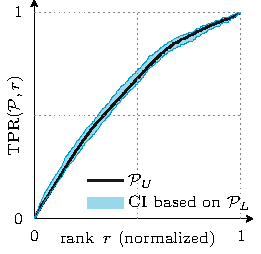
\includegraphics[width=0.25\textwidth]{covtype_cdf.pdf}}\qquad
\subfigure[ROC curves.\label{fig:results-covtype-roc}]{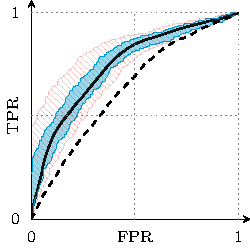
\includegraphics[width=0.25\textwidth]{covtype_roc.pdf}}\qquad
\subfigure[PR curves.\label{fig:results-covtype-pr}]{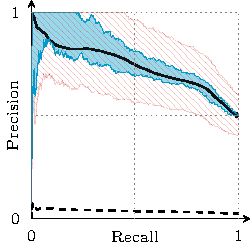
\includegraphics[width=0.25\textwidth]{covtype_pr.pdf}}
\addtolength{\abovecaptionskip}{-3mm}
%\subfigure[Rank CDF for \sensit.]{\includegraphics[width=0.29\textwidth]{cdf_sensit_2_semi_resvm.pdf}}\qquad
%\subfigure[ROC curves for \sensit.]{\includegraphics[width=0.29\textwidth]{roc_sensit_2_semi_resvm.pdf}}\qquad
%\subfigure[PR curves for \sensit.]{\includegraphics[width=0.29\textwidth]{pr_sensit_2_semi_resvm.pdf}}
%\caption{Results for \covtype and \sensit showing rank CDF, ROC and PR curves (left to right).}
\caption[]{Results for \covtype showing rank CDF, ROC and PR curves, with $\pfrac\approx 49\%$. \newline
Performance curve legend: 
\begin{tikzpicture}[baseline=-0.5ex] \draw [color=black, thick] (0, 0) -- (0.5, 0); \end{tikzpicture} true curve, 
\begin{tikzpicture}[baseline=-0.5ex] \draw [color=black, thick, dashed] (0, 0) -- (0.5, 0); \end{tikzpicture} $\hat{\pfrac}=0$, 

\begin{tikzpicture}[baseline=-0.5ex] \draw [color=cyan!80!black, opacity=0.8] (0, -0.2) rectangle (0.7, 0.3); 
\fill [color=cyan!80!black, opacity=0.4] (0, -0.2) rectangle (0.7, 0.3); \end{tikzpicture} $\hat{\pfrac}=\pfrac$ and 
\begin{tikzpicture}[baseline=-0.5ex] \draw [color=red!80!black, opacity=0.2, pattern=north west lines, pattern color=red!80!black] (0, -0.2) rectangle (0.7, 0.3); \end{tikzpicture} $0.8\pfrac \leq \hat{\pfrac} \leq 1.2\pfrac$.}
\label{fig:results-covtype}
\addtolength{\abovecaptionskip}{3mm}
\end{figure}

%%%%%%%%%%%%%%%%%%%%%%%%%%%%%%%%%%%%%%%%%%%%%%%%%%
%%%%%%%%%%%%%%%%%%%%%%%%%%%%%%%%%%%%%%%%%%%%%%%%%%
%
% 	Conclusion
%
%%%%%%%%%%%%%%%%%%%%%%%%%%%%%%%%%%%%%%%%%%%%%%%%%%
%%%%%%%%%%%%%%%%%%%%%%%%%%%%%%%%%%%%%%%%%%%%%%%%%%

\section{Conclusion}
We presented an approach to compute contingency tables corresponding to a lower and upper bound on FPR at a given rank based on a confidence interval on the rank CDF of (known) positives. Via these estimated contingency tables many commonly used performance metrics become available in a semi-supervised setting. We have shown that the bounds enable proper model evaluation, though model selection based on AUROC requires good estimates of the fraction of latent positives in the unlabeled set ($\pfrac$). Poor estimates of $\pfrac$ may invalidate the bounds and hamper model selection.

Our approach was used to compute bounds on ROC and PR curves in a realistic experiment, the quality of which is limited only by the quality of estimated confidence intervals on the CDF of ranks of positives and the estimated fraction of latent positives $\hat{\pfrac}$. Due to the sensitivity of the bounds in PR space to $\hat{\pfrac}$, we recommend using ROC curves for model evaluation in a partial labeling context. % unless $\hat{\pfrac}$ is known to be good estimate. %The proposed bounds enable thorough model assessment in a semi-supervised setting.% and hence address an important practical problem.
